% ------------------------------------------------------------------------ %
% !TEX encoding = UTF-8 Unicode
% !TEX TS-program = pdflatex
% !TEX root = ../Tesi.tex
% !TEX spellcheck = it-IT
% ------------------------------------------------------------------------ %
%
% ------------------------------------------------------------------------ %
% 	introduction
% ------------------------------------------------------------------------ %
%

\cleardoublepage
%
\phantomsection
%
%\addcontentsline{toc}{chapter}{Introduction}
%
\chapter{Introduction}
%
%\markboth{Introduction}{Introduction}	% headings
%
\label{cap:introduction}

\section{High Performance Computing}
The term High Performance Computing (HPC) refers to the use of supercomputers in order to solve computational problems either too complex to be solved by standard machines or extremely expensive in terms of time. Supercomputers are clusters of nodes, provided with a number of processors able to communicate with each other and to share resources as efficiently as possible.

Nowadays, with the growing number of large-scale simulations and data-intensive critical applications, e.g. deep learning training models, HPC plays an increasingly important role in many application areas \cite{marqube_2020}.

More and more often, HPC systems complement the use of traditional CPUs with accelerators such as GPUs, which offer a huge processing power thanks to the large number of cores, and FPGA, which can be adapted to specific tasks, favoring the heterogeneity of the system itself.

However, the technology enhancement, the increasing number of nodes and the loss of Dennard scaling \cite{10.1145/2024723.2000108} are introducing many challenges in power distribution and dissipation \cite{article}, dependability and resilience \cite{inproceedings}, resource allocation scheduling \cite{4629245} and parallel programming models \cite{Shalf2010ExascaleCT}.

\subsection{HPC Systems Architectures}
Intel distinguishes three main classes of HPC design, depending on the application area \cite{intel}:
\begin{description}
\item [Parallel Computing.] It aggregates the computing power of dozens or hundreds of processors located in a single physical system executing calculations simultaneously. It allows the computation of big and complex problems, splitting the workload into separate tasks carried out simultaneously.
\item [Cluster Computing.] It combines the processing capability of many independent computers linked together through a local-area network (LAN), acting like a single one. This configuration aims to solve a single problem spanning it across the nodes of the system, defining a specific network topology and organization in order to maximize the processing speed.
\item [Grid/Distributed Computing.] It connects multiple computers through a network to solve a complex problem or performing a large computational task. This approach allows to address jobs that can be split into separate chunks and distributed across the grid. Each node performs tasks independently without the need of communicating with the other nodes. 
\end{description}

\begin{figure}[t]
    \centering
    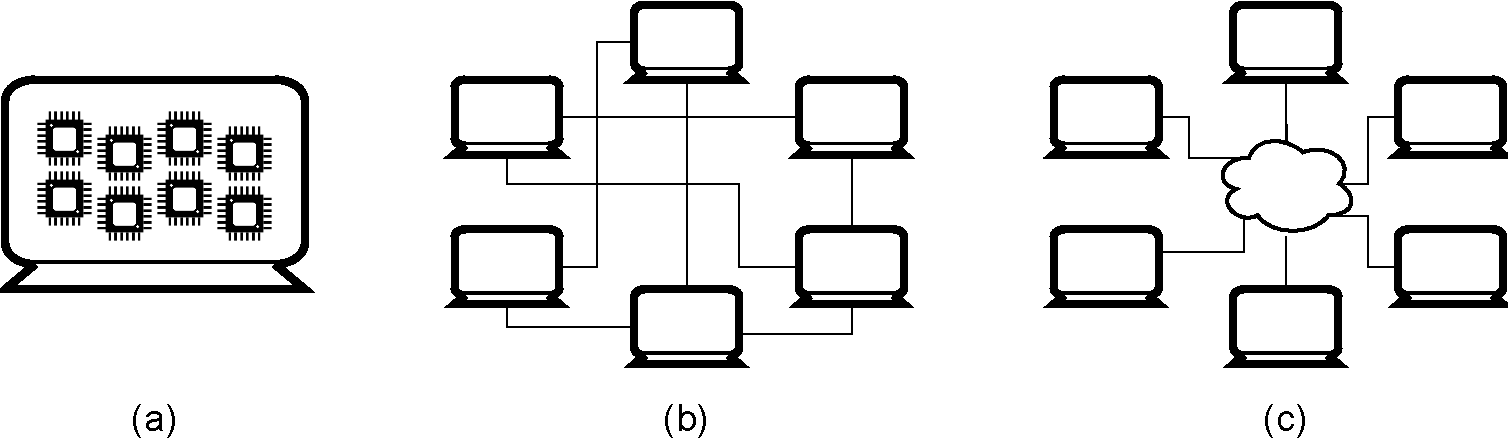
\includegraphics[width=\textwidth]{HPC_architectures.pdf}
    \caption{HPC system architectures: (a) Parallel Computing, (b) Cluster Computing, (c) Grid/Distributed Computing.}
    \label{fig:hpcarch}
\end{figure}

It becomes clear that architectural choices, including the hardware components to employ, play a fundamental role in the design of a HPC system.

At the time of writing, on one hand, Intel proposes the 3rd generation of Xeon Scalable processors. More specifically, Intel Xeon Platinum 8300 processors, the HPC flagship line of the company, offers up to 28 cores with the highest supported frequency of 4.3 GHz.

On the other hand, AMD, with its 2nd generation of EPYC High frequency processors, offers up to 64 cores with the highest supported frequency of 3.4GHz. Both solutions are provided with a DDR4 with the highest memory speed of 3200 MT/s.

With respect to the communication, in HPC systems, the nodes are usually connected via high speed networks, typically 10Gigabit Fiber Optics Ethernet or InfiniBand, which is used for data interconnect both among and within computers.

Storage is also a major matter of focus: Network Attached Storage (NAS) and Storage Area Network (SAN) are currently the most used solutions. NAS allows data to be stored in a centralized fashion in order to be accessible by all the nodes of the network and supports Redundant Array of Independent Disks (RAID) solutions to ensure data security. While NAS focuses on ease of use, manageability and scalability, SAN points its attention to high performance, low latency and lower total cost of ownership. It offers any-to-any connectivity among servers and storage devices, improving backups and redundancy. Either way, it is important that storage performance and capacity scale linearly with the numbers of nodes and disks.

\section{Reliability in HPC Systems}
With the arrival of exascale-grade High Performance Computing \cite{10.1145/3372390}, reliability becomes a matter of big concern at different scales: failures and downtimes have a severe impact on the performance of parallel programs, while the presence of a multitude of hardware and software components make failure and reliability prediction a challenging problem \cite{4629245}. 

Reliability concerns affect not only supercomputers but also data centers. More advanced technologies with higher susceptibility to radiation and aging, the use of larger memories, as well as the effect of other semiconductor components, such as processors and GPUs, can only lead to much higher hardware-related failure rates in the future \cite{10.1145/3403956}.
In the next paragraphs, the terminology of the paper \textit{Dependable Computing and Fault Tolerance: Concepts and Terminology} \cite{532603} will be followed to address  the various attributes of computing systems dependability.

\subsection{Faults, errors and failures}
A \emph{fault} is defined as the cause originating one or several latent \emph{errors} in the component where it occurs. An example of fault might be a programmer's mistake or a short occurring in an integrated circuit causing a connection stuck at a Boolean value. At some point, the latent error might be activated, becoming effective, and it might propagate from one component to another. Keeping on the examples above, the error in the written software or the stuck-at fault may become effective through the activation of the module in which the error resides, determining a mistaken output. A \emph{failure} occurs when the dysfunctions in the underlying architecture begin to deviate the behavior of higher-level modules, affecting the delivered service. Figure~\ref{fig:chain} summarize what Avizienis et al. \cite{1335465} define as the \emph{fundamental chain of dependability and security threats}: white arrows express causality relationship between fault, errors and failure. 

From the failure domain viewpoint, one can distinguish between:
\begin{figure}
    \centering
    
\includegraphics[width=\textwidth]{fault_error_failure.pdf}
    \caption{The fundamental chain of dependability and security threats.}
    \label{fig:chain}
\end{figure}
\begin{description}
    \item [Content failures.] Deviation of the content of the information from the golden (non-faulty) execution.
    \item [Timing failures.] Arrival time and/or duration of the execution different from the golden one. They can be distinguished in \emph{early} and \emph{late} depending on when the service is delivered.
\end{description}

Failures where both content and timing constraints are not satisfied fall in two classes:
\begin{description}
\item[Halt failures.] The service is halted, system activity is no longer observable by the user, external state becomes constant.
\item[Erratic failures.] The provided service is erratic and/or under-performing.
\end{description}
\begin{figure}[t]
    \centering
    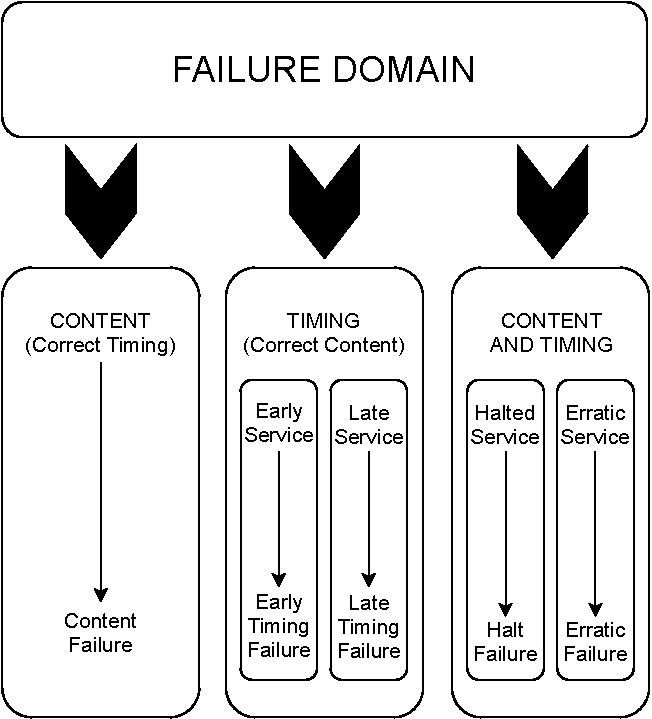
\includegraphics[width=0.7\textwidth]{failure_domain.pdf}
    \caption{Service failure modes with respect to the failure domain viewpoint.}
    \label{fig:failure_domain}
\end{figure}
Figure~\ref{fig:failure_domain} summarizes the service failure modes with respect to the failure domain viewpoint.

Both timing and/or content errors can be classified in the following categories:
\begin{description}
    \item [Silent Data Corruption (SDC).] The error is not detected but data is corrupted.
    \item [Detected Unrecoverable Error (DUE).] The error is detected, but it cannot be corrected.
    \item [Corrected Errors (CE).] The error is corrected and content and timing are recovered.
\end{description}

\subsection{Fault sources in HPC}
Reliability has been acknowledged as a major roadblock for HPC applications in current supercomputers and data centers. Although solution to ensure fault tolerance have been already developed, faults are still a huge source of issues in nowadays HPC systems.

As the HPC centers get larger, the probability of errors increases proportionally to the number of components \cite{10.1145/3403956}. Moreover, miniaturization causes smaller devices to be subject to increasing current densities at relatively high temperatures. In this scenario, thermal aging becomes a major concern: Bias Temperature Instability (BTI), is one of the most relevant aging effects in CMOS technology \cite{10.1145/3403956}. A sudden increase in temperature might result in charges being trapped in the transistor gate oxide reducing the voltage threshold of the transistors consequently affecting the maximum frequency of the circuit. BTI not only generates a faulty transient effect, present until the system is switched off, but also increases the probability and intensity of this effect as the system ages. In recent years, more and more HPC applications need strict timing requirements which would be endangered by this problem \cite{reghenzani2020timing}.

Canal et al. in \cite{10.1145/3403956} explains how thermal stress reduces the Mean Time To Failure (MTTF) of the system, but reducing hot spots is a not sufficient solution to cope with high performance CPUs thermal management: dynamic behaviors of temperature, summarized below, have a strong impact on the reliability of HPC processors and need to be taken into account.
\begin{description}
\item[Temporal Temperature Gradient (TTG).] Defined as the rate in which temperature changes over time, it depends on the workload capacity of each processing element and its operating frequency. It has a severe impact on the lifetime of the system.
\item[Spatial Temperature Gradient (STG).] It is the difference in temperature between two distinct points of the circuit. It also affect the system lifetime reliability, but, differently from TTG, it is mostly caused by power and thermal throttling at processor level.
\item[Thermal Cycling (TC).] As the name suggests, it consists in a periodic increasing and decreasing of the circuit temperature. It may be caused by power saving techniques as Dynamic Voltage and Frequency Scaling (DVFS) or the switching on and off of the processing elements. It poses a more serious impact on the MTTF as the amplitude of the cycles increases.
\end{description}

\subsection{The heterogeneity challenge}
HPC systems revealed themselves as a fundamental instrument in the resolution of problems in a variety of scientific fields, supporting research and innovation  by increasing exploration speed and effectiveness, nevertheless, the demand for a higher-performance supercomputer keeps increasing \cite{10.1145/3372790}. Particularly, the importance of heterogeneity is sensibly growing. The introduction and diffusion of GPUs as processing units is leaving a great mark in the performance of parallel computing, such that it is reasonable to think that they will be more and more used in the future. Originally, GPUs had been designed to improve image rendering, a field of application in which reliability was not a topic of main importance, since it was intrinsically fault tolerant \cite{Fang12evaluatingthe}. However, in the recent years, General Purpose GPUs (GPGPUs) are becoming a powerful resource in HPC systems, where the complexity of the hardware and the extensive number of components  considerably enlarges the probability of failures, making indispensable a concern in such regard.

Cini et al., in \cite{10.1145/3372790}, listed a series of reasons why heterogeneous systems, more specifically GPU based, are less reliable than homogeneous ones, CPU based:
\begin{description}
\item [Massive Parallelism.] An application running on a GPU can consists of millions of independent thread which means that the failure of one of them does not affect any of the others. The problem is that an error can propagates very quickly if not detected in time and, if it lies on shared resources, it may affect also other nodes. In this circumstances, a failure is very costly compared to an homogeneous system. Moreover, experimental studies show that memory errors are likely to disturb multiple threads or multiple thread blocks.
\item[High Density.] Since a GPU is made up of a large number of execution units (EUs) it may reach a very high temperature. If a 12-core CPU contains about 72 EUs, GPUs can consist of more than 3000 EUs, which, if working in parallel, might cause the system to overheat with a probability of causing failures 10x higher than CPUs.
\item[High Utilization.] The number of GPUs is growing in heterogeneous systems and the huge number of cores makes systems more susceptible to failures. Furthermore, applications running on GPUs are destined to become increasingly popular, intensifying the utilization and, consequently, the error rate. 
\end{description}

Beside GPU accelerators technology, architectural specialization is another exploited option in HPC to face the slow down in Moore’s Law: in recent years, the use of FPGA technology is catching on to improve performance and lower energy costs \cite{insidehpc_2019}. Edward Stott et al., in \cite{5694288}, identify Negative-Bias Temperature Instability (NBTI) the primary degradation mechanism of FPGA, finding that the generated wear out speed strongly depends on the supply voltage and temperature. 
Amouri et al. carried out an experimental analysis \cite{6927390}, from which resulted that after just one week of  continuous stress, FPGA had shown an aging extent of up to 5.17\%, correlating the problem to the effect of the Input Signal Probability (SP) and the effect of the Switching Activity (SA).

As shown, the progress in HPC systems comes with the need of a particular attention to the problem of the reliability towards the hardware components that constitute them and, consequently, towards the applications that run on them, which is the main concern at the base of the presented work. 

\section{Thesis objectives and structure}
This thesis work aims to cope at software level with the reliability issues of HPC systems, through the design, implementation and integration in the BarbequeRTRM of a scheduling policy able to proactively minimize the degradation of the hardware components, while ensuring a backup plan in case of occurrence of failures. This purpose will be achieved taking care as much as possible of the reliability-performance trade off and exploiting a resource allocation algorithm, able to adapt itself not only to the specific machine in which it runs, but also to the process to execute. 

The thesis is organized as it follows: 
\begin{description}
\item[{\hyperref[cap:stateofart]{State of the Art.}}] In this chapter an overview on the Checkpoint/Restart technique and the Run Time Resource Managers, pillars on which the project presented by this thesis is built, is given, highlighting the limits of the state of the art.
\item[{\hyperref[cap:implementation]{Design and Implementation.}}] In this chapter the design and the implementation of the Dynamic Checkpoint Rate Tuning and of the Reliam Resource Allocation Policy, the two main components of this work, are deeply examined, with a focus on the framework in which they have been integrated, i.e. the BarbequeRTRM.
\item[{\hyperref[cap:experimental]{Experimental Evaluation.}}] In this chapter the series of experiments performed on the Dynamic Checkpoint Rate Tuning and on the Reliam Resource Allocation Policy will be described, analyzed and commented. Through those tests, not only a measurement of the effectiveness of the proposed work will be extract, but also some guideline in the choice of the parameters at users discretion.
\end{description}